% Options for packages loaded elsewhere
\PassOptionsToPackage{unicode}{hyperref}
\PassOptionsToPackage{hyphens}{url}
%
\documentclass[
]{book}
\title{A Minimal Book Example}
\author{John Doe}
\date{2021-12-01}

\usepackage{amsmath,amssymb}
\usepackage{lmodern}
\usepackage{iftex}
\ifPDFTeX
  \usepackage[T1]{fontenc}
  \usepackage[utf8]{inputenc}
  \usepackage{textcomp} % provide euro and other symbols
\else % if luatex or xetex
  \usepackage{unicode-math}
  \defaultfontfeatures{Scale=MatchLowercase}
  \defaultfontfeatures[\rmfamily]{Ligatures=TeX,Scale=1}
\fi
% Use upquote if available, for straight quotes in verbatim environments
\IfFileExists{upquote.sty}{\usepackage{upquote}}{}
\IfFileExists{microtype.sty}{% use microtype if available
  \usepackage[]{microtype}
  \UseMicrotypeSet[protrusion]{basicmath} % disable protrusion for tt fonts
}{}
\makeatletter
\@ifundefined{KOMAClassName}{% if non-KOMA class
  \IfFileExists{parskip.sty}{%
    \usepackage{parskip}
  }{% else
    \setlength{\parindent}{0pt}
    \setlength{\parskip}{6pt plus 2pt minus 1pt}}
}{% if KOMA class
  \KOMAoptions{parskip=half}}
\makeatother
\usepackage{xcolor}
\IfFileExists{xurl.sty}{\usepackage{xurl}}{} % add URL line breaks if available
\IfFileExists{bookmark.sty}{\usepackage{bookmark}}{\usepackage{hyperref}}
\hypersetup{
  pdftitle={A Minimal Book Example},
  pdfauthor={John Doe},
  hidelinks,
  pdfcreator={LaTeX via pandoc}}
\urlstyle{same} % disable monospaced font for URLs
\usepackage{longtable,booktabs,array}
\usepackage{calc} % for calculating minipage widths
% Correct order of tables after \paragraph or \subparagraph
\usepackage{etoolbox}
\makeatletter
\patchcmd\longtable{\par}{\if@noskipsec\mbox{}\fi\par}{}{}
\makeatother
% Allow footnotes in longtable head/foot
\IfFileExists{footnotehyper.sty}{\usepackage{footnotehyper}}{\usepackage{footnote}}
\makesavenoteenv{longtable}
\usepackage{graphicx}
\makeatletter
\def\maxwidth{\ifdim\Gin@nat@width>\linewidth\linewidth\else\Gin@nat@width\fi}
\def\maxheight{\ifdim\Gin@nat@height>\textheight\textheight\else\Gin@nat@height\fi}
\makeatother
% Scale images if necessary, so that they will not overflow the page
% margins by default, and it is still possible to overwrite the defaults
% using explicit options in \includegraphics[width, height, ...]{}
\setkeys{Gin}{width=\maxwidth,height=\maxheight,keepaspectratio}
% Set default figure placement to htbp
\makeatletter
\def\fps@figure{htbp}
\makeatother
\setlength{\emergencystretch}{3em} % prevent overfull lines
\providecommand{\tightlist}{%
  \setlength{\itemsep}{0pt}\setlength{\parskip}{0pt}}
\setcounter{secnumdepth}{5}
\usepackage{booktabs}
\ifLuaTeX
  \usepackage{selnolig}  % disable illegal ligatures
\fi
\usepackage[]{natbib}
\bibliographystyle{plainnat}

\begin{document}
\maketitle

{
\setcounter{tocdepth}{1}
\tableofcontents
}
\hypertarget{arbeidskrav1}{%
\chapter{Arbeidskrav1}\label{arbeidskrav1}}

\hypertarget{introduksjon}{%
\section{Introduksjon}\label{introduksjon}}

En av de mest sentrale faktorene for utholdenhets prestasjonen er det maksimale oksygenopptaket (VO2maks) \citet{bassett2000}. VO2maks er bestemt av flere sentrale faktorer: lungenes kapasitet til å føre oksygen fra blodet, hjertets pumpekapasitet, volum, og sammensetning av blodet, og musklenes evne til å bruke oksygenet \citet{bassett2000}.

Reliabilitet kan bli definert som reproduserbarheten til testverdier, analyser eller andre målinger på gjentatte forsøk på de samme individene. Det finnes tre hoved variasjoner man må ta hensyn til når man snakker om reliabilitet, det er: deltakernes variasjon, endring i gjennomsnittet og rettest korrelasjon \citet{hopkins2000}. Deltakernes variasjon regnes ut gjennom standardavvik og standardfeil. Det kan komme fra biologiske forhold som kan variere mellom to tester. Utstyr kan og spille inn på dette, hvor det er støy ved målingene. Endring i gjennomsnitt kan man dele i to deler, det er tilfeldig endring og systematisk endring. Tilfeldig endring er støy i målinger og data innsamlingsfeil. Dette kan minimeres gjennom å ha mange tester, hvor da tilfeldige feilene vil spille mindre inn på resultatet. Systematisk endring er treningseffekten og læringseffekten man kan forvente mellom to tester, det handler om faktorene som spiller inn og kan gjøre test2, bedre enn test1. Korrelasjon i test2 handler om hvor godt test1 og test2 korrelerer, hvis man har bedre korrelasjon, har man og høyere reliabilitet mellom testene.

\hypertarget{metode}{%
\section{Metode}\label{metode}}

I denne rapporten skal reliabiliteten estimeres mellom to VO2maks tester. Hvor test1 og test2 er gjennomført med en ukes mellomrom.

VO2maks testen ble gjennomført med en standard VO2maks protokoll. Hvor stigningen var konstant, 10,5\% for guttene og 5,5\% for jentene. Startfart var gitt på forhånd hvor alle startet på 8 km/t. For hvert minutt som gikk, økte farten med 1 km/t, og slik fortsatte det til utmattelse. Underveis i testen ble det gitt verbal oppmuntring fra testleder, det var og testleder som justerte farten underveis. Testen ble gjennomført på en woodway løpemølle (4FRONT, wisconsin). Hele testen ble gjennomført med kontinuerlig oksygenmåling hvert 30. sekund. Oksygenmålingene ble gjennomført med en Vyntus CPX, mixing chamber (Vyntus CPX, Jaeger-CareFusion, UK). Ved målinger på Vyntus CPX ble det automatisk kalibrert for gass, volum og luftfuktighet før hver test. Oppvarmingen før testen var valgfri, og varte i 15 min. Underveis i oppvarmingen ble testprotokollen forklart for utøver, og eventuelle spørsmål om testen ble avklart. Under testen ble det registrert ml/min VO2. Umiddelbart etter testen ble det spurt om Borg skala 6-20 (RPE: \citet{borg1970} ), det ble og notert ned hva siste belastning var og hvor lenge utøver løp på denne belastningen. Et minutt etter testen ble det målt laktat (La) gjennom et fingerstikk og analysert gjennom Biosen blodlaktatmåler (Biosen C-line, EKF Diagnostics, Barleben, Germany), HF ble og notert ned.

Test2 ble gjennomført på samme måte som test1, hvor samme protokoll ble gjennomført på nytt.

\hypertarget{statistikk}{%
\section{Statistikk}\label{statistikk}}

Alle statistiske beregninger ble gjort i RStudio (versjon RStudio 1.4.1717; R Foundation for Statistics Computing, Vienna, AT). Det ble regnet ut gjennomsnitt og standardavvik mellom test1 og test2. Det ble også regnet ut standardfeil for testen som et mål på reliabilitet.

\hypertarget{resultat-og-diskusjon}{%
\section{Resultat og diskusjon}\label{resultat-og-diskusjon}}

Resultatene for studien er vist i figur 1.

Standardfeilen i studien var 4.04 \%.

Standardaviket i studien var 229.82

\begin{figure}
\centering
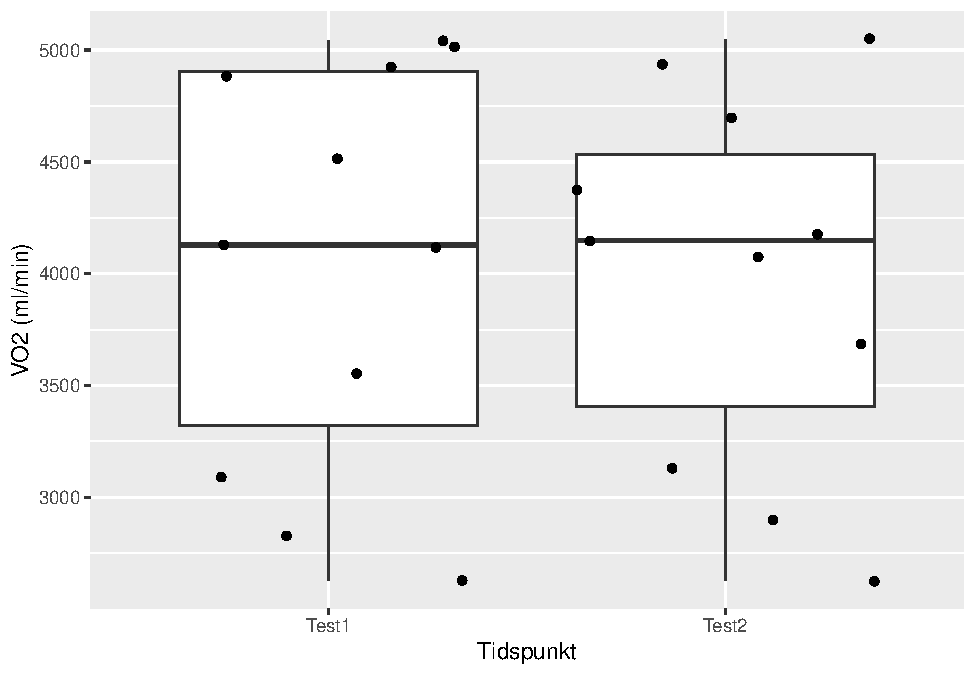
\includegraphics{_main_files/figure-latex/unnamed-chunk-2-1.pdf}
\caption{\label{fig:unnamed-chunk-2}Figur 1 viser resultater fra test 1 og 2}
\end{figure}

\hypertarget{vitenskapsfilosofi}{%
\chapter{Vitenskapsfilosofi}\label{vitenskapsfilosofi}}

\hypertarget{falsifikasjonisme}{%
\section{Falsifikasjonisme}\label{falsifikasjonisme}}

Hva er Poppers falsifiserbarhetskriterium og hvilket spørsmål skal dette kriterium gi svar på?
Hvorfor mener andre vitenskapsfilosofer (f.eks. Okasha) at vi ikke trenger å svare på dette spørsmålet?
Hvem synes dere har rett?

Poppers falsifiserbarhetskriterium handler enkelt forklart om hva han mente var en god vitenskapelig teori og hva som var en dårlig.
I følge Popper ville det å si at noe var en god vitenskapelig teori bety at den var falsifiserbar \citet{okasha2016}.
At en teori er falsifiserbar, betyr at det skal være mulig å påvise at den er gal eller uholdbar, og er det motsatte av å kunne verifisere.
I følge popper var det en skarp linje mellom vitenskapelige og uvitenskapelige teorier, altså falsifiserbare og ufalsifiserbare teorier \citet{okasha2016}.
Og at vitenskapelige teorier ikke kunne bli bekreftet, hverken godt eller dårlig de kan kun bli falsifisert og aldri bekreftet \citet{okasha2016}.
Med dette mente popper at man kunne unngå induksjonsproblemet, som er hvordan man skal begrunne gyldigheten til teorier \citet{okasha2016}.
For hvis man isteden bare prøvde å falsifisere dem var det ingen grunn til å bruke induksjon.
Bakgrunnen for falsifiserbarhetskriteriet til popper var også at det skulle gi et svar på demarkasjonsproblemet, som er spørsmålet om hva som egentlig skiller vitenskap fra ikkevitenskap.

Den logiske strukturen til poppers falsifisering er at fra en teori kan vi utarbeide hypoteser, hvis disse hypotesene viser seg å være usanne via observasjoner og eksperimenter, vil dette bety at teorien er usann \citet{okasha2016}.
En falsifiserbar teori vil da stride med noen mulige empiriske observasjoner, den vil også gi gode forutsigelser, altså forutsigelser som kan bli testet mot data og som ville falsifisere teorier hvis ikke dataen stemmer med forutsigelsen \citet{okasha2016}.
En ufalsifiserbar teori vil derimot være forenlig med alle mulige empiriske observasjoner, og den vil ikke gjøre noen forutsigelser som kan testes mot dataen og dermed kunne falsifisere teorien dersom dataen ikke passet med forutsigelsen \citet{okasha2016}.

Andre vitenskapsteorier mener at det ikke er en skarp linje mellom vitenskapelige og uvitenskapelige teorier.
Derimot er den viktigste forskjellen mellom godt og dårlig bekreftede teorier.
Spesielt \citet{okasha2016} mente at svakheten i Poppers argument var klar.
For målet med vitenskapen er ikke bare å motbevise teorier, men også anta hvilke teorier som er sanne eller mest sannsynlig sanne.
Han foreslo at når vitenskapsmenn samler data vil kanskje målet deres være å vise at en spesiell teori, muligens fra deres erkerival, er feil.
Men mer sannsynlig prøver de å bevise at deres egen teori er sann.
Og for å kunne gjøre dette må de muligens ty til en form for induktivt argument.
Så Poppers forsøk på å vise at vitenskap kan klare seg uten induksjon lykkes ikke.
Slik jeg ser det veldig vanskelig å avgjøre hvem jeg syns har rett, jeg syns at popper har et veldig godt poeng med å ha et falsifiseringskriterium og et skarpt skille mellom hva som er vitenskap og ikke.
Ved dette vil det bli veldig klart hva som er vitenskap og det kan være en stor fordel.
Samtidig er det ikke helt riktig å dra all vitenskap som ikke kan falsifiseres under en kam og kalle det for psudo- vitenskap, eller ikke vitenskap.
Så jeg syns det er vanskelig å gjøre meg opp en klar mening om hvem som har rett når jeg syns begge to har gode meninger.

\hypertarget{hd-metoden-og-abduksjonbayesisme}{%
\section{HD-metoden og abduksjon/Bayesisme}\label{hd-metoden-og-abduksjonbayesisme}}

Hva er strukturen på et bekreftende vitenskapelig argument ifølge den hypotetisk deduktive metode?
Forklar ut fra Hempels artikkel men bruk egne eksempel.
Sammenlign også Hempels HD-metode med hvordan vitenskapelig bekreftelse fungerer ifølge enten abduksjon eller Bayesianisme.

Hypotetisk deduktiv metode, eller HD- metoden har en struktur som bekrefter vitenskapelige argumenter gjennom å få positive resultater når man tester de deduktive konsekvensene av teorien \citet{hempel1966}.
Strukturen til HD- metoden er beskrevet av Hempel \citet{hempel1966}, det første trinnet i HD- metodens strukturen er en «utdannet gjetning», her blir det formulert en hypotese eller teori.
I det andre trinnet i strukturen blir det utledet empiriske konsekvenser fra teorien eller hypotesen.
Testingen eller observasjoner av disse empiristiske konsekvensene skjer i trinn tre.
Og i trinn fire ser man på om de empiriske konsekvensene viser seg å være riktige, og da blir teorien bekreftet til en viss grad, på induktivt vis.
Hvis jeg skal forklare HD- metoden ved et eget eksempel kan jeg stille et spørsmål som «hvordan kan vi vite at kyssesyken er et virus?»
I trinn to, vil i så fall da kyssesyken (a) være smittsom, men (b) ikke bli kurert av antibiotika.
I trinn tre, vil observasjoner og eksperimenter vise at kyssesyken både er (a) og (b).
Derfor vil vi i trinn fire kunne få en induktiv bekreftelse på at kyssesyken er forsaket av et virus.

En annen form for vitenskapelig bekreftelse som er interessant å sammenligne med den hypotetiske deduktive metoden er bayesianisme.
Bayesianisme er en metode som brukes for å øke tillitten til en teori eller hypotese ettersom mer informasjon og bevis blir tilgjengelige \citet{okasha2016}.
For å få til dette brukes det sannsynlighet, ifølge bayesianisme må en rasjonell person meninger om hvor sannsynlig forskjellige påstander er.
Dette betyr at om en forsker er 50\% sikker på at en teori er riktig må man også være 50\% sikker på at teorien er usann.
Sannsynligheten kommer ut i fra at forskere bruker den bayesiske kondisjonaliseringsregelen, som sier at når en har hentet inn data(D), burde sannsynlighetsverdiene for en teori(T) oppdateres gjennom å kondisjonalisere D.
Og T burde da aksepteres som bekreftet når sannsynligheten er tilstrekkelig høy \citet{okasha2016}.
Et eksempel på bayeiansisme i praksis blir beskrevet av Okasha \citet{okasha2016} som følger, hvis vi ser for oss at en T har et testbart utsagn (U), og forskeren i utgangspunktet har tillit til at både T og U er sant.
Vi antar at både T og U tar «non- extreme values», som vil si at de verken er en eller null.
Hvis vi deretter ser for at forskeren finner ut at U er definitivt sant, vil det være logisk at forskeren får en enda større tro på at T også er sann.
Med andre ord en forsker som oppdager at teorien deres har gitt en sann spådom vil nødvendigvis øke deres tillitt til teorien så lenge de adlyder kondisjonaliseringsregelen.
Så det faktum at suksessfulle utsagn ofte fører til at forskere får mer tiltro til deres egen teori, har en ryddig forklaring på det bayesianske synet på vitenskapelig bekreftelse \citet{okasha2016}.
Hovedforskjellen mellom hypotetisk deduktiv metode og bayesisme er da at HD- metoden tar en utdannet gjetting i forhold til observasjonene den får inn, mens bayesisme bare blir styrket mer og mer etter som den får inn flere resultater og tilslutt blir bekreftet når sannsynligheten er høy nok.
Begge metodene tar også en bekreftelse ut fra resultatene de kommer frem til, men HD- metoden har på forhånd en hypotese den tester ut ifra, som eksemplet mitt viste hvor hypotesen var at kyssesyken var et virus.
I HD- metoden blir da eksperimentene og forskningen testet for å bekrefte eller motbevise dette, mens i bayesismen vil da teorien til forskerne kunne endres mye underveis ettersom hvilke resultater de kommer frem til.

\hypertarget{replikasjonskrisen}{%
\section{Replikasjonskrisen}\label{replikasjonskrisen}}

Hva mener Alexander Bird er forklaringen til at mange resultat i noen vitenskaper ikke repliseres?
Oppsummere Birds argument for dette.
Sammenlign også Birds forklaring med noen av de andre forklaringene som Bird diskuterer i seksjon 4.
Har Bird rett i at hans forklaring er bedre?

Begrepet replikasjonskrisen er brukt til å beskrive både at det er enormt mange felt av studier det ikke er mulig å replisere, og at disse feltene står ovenfor en krise som en konsekvens av dette \citet{bird2020}.
Ut av 1576 forskere i en undersøkelse mener hele 52\% at det er en signifikant krise når det kommer til replikasjon \citet{baker2016} .
En spesiell bekymring av replikasjonskrisen er at det vil muligens øke mistillit til vitenskapen som tilhører helt andre felt enn der selve replikasjonskrisen oppstår \citet{bird2020}.\\
Grunnen til at mange resultater innenfor forskingen ikke kan repliseres er på grunn av basefrekvensfeilen, her er det to typer feil, akseptere en usann teori og avise en sann teori.
Bird \citet{bird2020} mener Basefrekvensfeilen vil gjerne oppstå når man trekker en slutning om sannsynligheten for en bestemt forekomst av et generelt fenomen, for eksempel om en person har en sykdom.
Feilslutningen oppstår når forskeren fokuserer utelukkende på et eller annet fremtredende bevis mens han overser hvor mange forekomster av dette fenomenet vil skje uansett, uavhengig av beviset.
Dette fører til feilaktige konklusjoner når bevisene er sterkt, men ikke helt korrekt, for eksempel når bevisene er en slags test for et fenomen, og selve fenomenet er sjeldent.
For å demonstrere dette bruker Bird et eksempel hvor passasjerer på et fly bli undersøkt for å være terrorister, hvor testen er 95\% riktig.
I dette tilfelle vil testen si at av 100 personer som ikke er terrorister vil 95 være ikke terrorist og 5 vil være terrorister.
I så fall om en person ikke består testen vil den si at han er en terrorist.
Dette mener Bird var tullete etter som det absolutt ikke var en så høy sannsynlighet for at passasjerer på fly er terrorister.
Hvis denne testen blir trodd vil det i så fall bli akseptert en usann teori.
Hvis mange av hypotesene vi tester er usanne, da er sannsynligheten til hypotesene som bekreftes i mange vitenskaper ganske lav \citet{bird2020}.
Andre forklaringer for replikasjonskrisen som Bird diskuterer er at enkelte har assosiert replikasjonskrisen med den lave statistiske kraften fra mange av studiene.
Populasjonen altså antall deltakere, styrer i stor grad styrken til forskningen, og gir en større sannsynlighet for å ikke få en type II feil, altså et falsk negativt resultat \citet{bird2020}.
Ifølge Bird er dette likevel ikke en god forklaring fordi man fremdeles får en høy sannsynlighet for type II feil selv med høy statistisk styrke \citet{bird2020}.
For å understreke dette viser Bird frem en utregning som tilsier at det fremdeles er 31\% sjanse for type II feil selv med høyere statistikk enn i «vanlig» vitenskap \citet{bird2020}.
Bird mener det dermed vil være en stor fordel for vitenskapen å få opp den statistiske styrken men det vil likevel ikke gi en løsning på krisen.\\
Basert det man har sett av studier er det vanskelig å gi en fast konklusjon men, dårlig praksis og juks kan være en forklaring på replikasjonskrisen \citet{bird2020}.
Derfor vil det ikke være gode nok argumenter til å mene at en dårlig moral innenfor vitenskapen kan forklare hele krisen \citet{bird2020}.
Slik jeg tolker det er det ganske tydelig at Bird mener hans egne argumenter og forklaring gir mest styrke til teorien om replikasjonskrisen.
Og en større forståelse av statistikk og sannsynlighet vil være viktig for alle som driver med vitenskap \citet{bird2020}.

\hypertarget{study-design}{%
\chapter{Study-Design}\label{study-design}}

\hypertarget{inntroduksjon}{%
\section{Inntroduksjon}\label{inntroduksjon}}

I denne oppgaven har jeg funnet 5 originalartikler \citep{billat2000, billat2001, dupont2002, thevenet2007, wakefield2009} som jeg skal sammenligne og se på hvordan design disse studiene har og hvilke statistiske analyser de bruker. Gjennom denne oppgaven ønsker jeg å fremheve hva studiene gjør bra og hva de eventuet kan gjøre bedre.

\hypertarget{metode-1}{%
\section{Metode}\label{metode-1}}

Formålet i alle studiene handler i hovedsak om å undersøke sammenhengen mellom intensitet ved kortintervaller og hor mye tid det gir over en gitt prosent av det maksimalt oksygenopptak (vo2 maks) deltakerne oppnår ved forskjellige protokoller. studien til \citet{thevenet2007} og \citet{wakefield2009} sammenligner begge effekten av treningsintensitet på tid over 95\% av VO2 maks, \citet{thevenet2007} har en hypotese som tilsier at en økning i hastigheten fra 100\% av farten ved vo2maks til 115\% av farten ved vo2maks under intervallene ville også gi en økning i tiden over 90- og 95\% av vo2maks. Mens \citet{wakefield2009} har en motsatt hypotese om at tid på eller over 95\% av vo2maks ville være lenger ved løp på 105\% av farten ved vo2 maks enn ved 115\% av farten ved vo2 maks. Studiene til \citet{billat2000} og \citet{billat2001} til forskjell intervaller hvor de ser på hvordan man kan fremkalle mest tid ved 100\% av vo2maks, deriblant hvilken intensitet og intervallform som er best for dette. Mens \citet{dupont2002} passer bra inn med alle de andre artiklene over og ser på både tid ved vo2maks og tiden over 90\% av vo2maks ved kortintervaller 15/15.

Alle studiene presenterte en hypotese. Hypotesen de kommer med er begrunnet av tidligere forskingsdata. Som et eksempel begrunner \citet{wakefield2009} sin hypotese ved å referere til data i studien til \citet{thevenet2007}. Gjennom å presentere denne dataen fra tidligere forskning skapes det en logisk linje gjennom introduksjonen til hypotesen. Dette blir gjort på en spesielt god måte i artikkelen til \citet{thevenet2007} hvor artikkelen starter bredt med å fortelle om vo2maks, og at det er ansett som en viktig faktor innenfor langdistanseløping. Dette blir bygget opp ved å referere til tidligere artikler som har kommet frem til dette. Videre blir det beskrevet treningsmetoder for å forbedre vo2maks, hvor mye tid på en høy \% av vo2maks blir beskrevet som en viktig faktor spesielt tid over 90- og 95\% av vo2maks. Etter dette beveger introduksjonen i artikkelen seg over på å fortelle om intervalltrening og spesielt kortintervaller og effekt på å kunne arbeide på en høy \% av vo2 maks. Artikkelen forteller videre om andre forskingsartikler som har sett på kortintervaller og tid over 90 og 95\% men avdekker samtidig kunnskapshull i disse artiklene. Dette gjør at \citet{thevenet2007} formulerer en hypotese basert på informasjonen om vo2maks og kortintervaller som skal forsøke å tette disse kunnskapshullene som ble beskrevet i introduksjonen.\\
Dermed funker denne introduksjonen som en trakt som starter med å fortelle om et tema bredt, og smaler seg etter hvert inn på mindre temaer og spesifikke problemer den ønsker å svare på, samtidig som den har en rød trå eller logisk linje gjennom introduksjonen og frem til hypotesen. De andre artiklene følger i likhet denne samme strukturen i sin innledning som leder til en hypotese.

Studiedesignet i alle disse studiene var randomisert kontrollert undersøkelse (RCT). I en RCT metode der sammenlignes flere grupper. Gruppene som sammenlignes burde være så like som mulig med tanke på alt som kan påvirke utfallet. Dette oppnås ved å tilfeldig fordele eller randomisere deltakerne.~I disse testene ble deltakerne randomisert i grupper som skulle utføre forskjellige intervaller eller så ble det randomisert rekkefølgen de skulle gjennomføre intervallene i. Denne randomisering er den metoden som med størst sannsynlighet gir sammenlignbare grupper.

Siden alle studiene på forhånd hadde spesifisert en primær hypotese stemmer dette også godt med designet i en clinical tril. En god regel for clinical trial, er å etablere flere hypoteser på forhånd som gir mening, men å spesifisere en hypotese som den primære, denne må kunne bli statistisk testet uten argument om at hyoptesen må endres (\citet{hulley2013} s53). Mer viktig vil en primær hypotese hjelpe studien å fokusere på dens hovedoppgaver og bidra til en ren base for kalkulasjoner av utvalgsstørrelsen (\citet{hulley2013} s53).

Alle studiene hadde en god beskrivelse av forsøkspersonene som var med i testen. De viste alle frem med standardavvik antall deltakere, kjønn, alder, høyde og vekt. Alle studiene fortalte også at alle deltakere var godt trente personer, at de hadde meldt seg som frivillige og at de var fullt informert over test prosedyren og hadde underskrevet på dette, foresatte underskrev for deltakere under 18 år. Alderen på deltakerne i de forskjellige studiene varierte mye hvor \citet{thevenet2007a} hadde den yngste snittalderen på 16,1± 1 mens \citet{billat2001} hadde den eldste snittalderen på 51±6. Ingen av disse to studiene forsvarte hvorfor de valgte å teste disse aldersgruppene på henholdsvis yngre og litt eldre utøvere.\\
I testen til \citet{thevenet2007} ble det forklart at deltakeren alle var rekruttert fra samme treningsklubb, og i studiene til både \citet{dupont2002} og \citet{wakefield2009} var deltakeren idrettsstudenter. I de to resterende artiklene var det ikke oppgitt hvor deltakerne var rekruttert fra \citet{billat2001} og \citet{billat2000} . Alle studiene hadde forholdsvis få deltakere med mellom 7-9 personer, og ingen av studien hadde noen forklaring på hvorfor de hadde det antallet deltakere. Dette er litt underlig ettersom en studie med flere deltakere ville gitt en større statistisk styrke, fordi det da vil være fler observasjoner som påvirker gjennomsnittet.\\
I alle studiene ble det brukt p-verdier som hvor signifikantnivået var P\textless0.05. ingen av studiene brukte andre tester som t- test eller effektstørrelse som kunne ha bidratt til å styrke resultatet ettersom dette er en test som kan styrke opp om p- verdien. Hvordan testene ble gjennomført var svært forskjellige \citet{wakefield2009} gjennomførte testen på mølle med 1\% stigning mens resten av testene ble gjennomført på løpe bane. Alle studiene hadde intervaller som en av testene, her var alle kortintervaller med mellom 15- 30sek arbeidstid. Før intervallene gjennomførte alle studiene vo2maks test, som ble bestemmende for farten de skulle løpe på under intervallene. \citet{dupont2002} hadde den raskeste hastigheten med 15/15s intervaller på 140\% av farten ved vo2maks, mens \citet{thevenet2007} hadde intervaller med lavest hastighet 30/30sek med 100\% av farten ved vo2maks. Under alle testene ble gassutveksling målt, dette innebar variabler som ventilasjon, pustefrekvens, oksygen, og co2. I tillegg målte alle studiene laktat mens \citet{billat2001} og \citet{billat2000} var de eneste som ikke målte hjertefrekvens. Av disse målingene var oksygenmålingen den eneste variabelen som direkte svarte på hypotesen i alle studiene.

\begin{longtable}[]{@{}
  >{\raggedright\arraybackslash}p{(\columnwidth - 4\tabcolsep) * \real{0.22}}
  >{\raggedright\arraybackslash}p{(\columnwidth - 4\tabcolsep) * \real{0.20}}
  >{\raggedright\arraybackslash}p{(\columnwidth - 4\tabcolsep) * \real{0.58}}@{}}
\toprule
\begin{minipage}[b]{\linewidth}\raggedright
Studie
\end{minipage} & \begin{minipage}[b]{\linewidth}\raggedright
Deltakere
\end{minipage} & \begin{minipage}[b]{\linewidth}\raggedright
Studiedesign
\end{minipage} \\
\midrule
\endhead
\citet{thevenet2007} & \begin{minipage}[t]{\linewidth}\raggedright
N= 9\\
Kjønn= M\\
Alder= 16,6±1\strut
\end{minipage} & \begin{minipage}[t]{\linewidth}\raggedright
RCT\\
Løpetest: 400m løpebane

Intervall 1: 30/30sek 100\% fart ved VO2maks

Intervall 2: 30/30sek\\
110\% fart ved VO2maks\strut
\end{minipage} \\
\citet{wakefield2009} & \begin{minipage}[t]{\linewidth}\raggedright
N= 7\\
Kjønn= M\\
Alder= 22 ± 5\strut
\end{minipage} & \begin{minipage}[t]{\linewidth}\raggedright
RCT\\
Løpetest: Løpemølle 1\% stigning

Intervall 1: 20/20sek på 105 og 115\%

Intervall 2: 25/20sek på 105 og 115\%

Intervall 3: 30/20sek på 105 og 115\%\strut
\end{minipage} \\
\citet{billat2001} & \begin{minipage}[t]{\linewidth}\raggedright
N= 7\\
Kjønn= M\\
Alder= 51±6\strut
\end{minipage} & \begin{minipage}[t]{\linewidth}\raggedright
RCT\\
Løpetest: 400m løpebane

Intervall 1: 15/15sek på 90-80\%

Intervall 2: 15/15sek på 100-70\%

Intervall 3: 15/15se på 60 x 110\%\strut
\end{minipage} \\
\citet{billat2000} & \begin{minipage}[t]{\linewidth}\raggedright
N= 8\\
Kjønn= M\\
Alder= 34±6\strut
\end{minipage} & \begin{minipage}[t]{\linewidth}\raggedright
RCT\\
Løpetest: 400m løpebane

Intervall 1: 30/30 sek på 100\%

Intervall 2: 30/30sek på laktattersekel\strut
\end{minipage} \\
\citet{dupont2002} & \begin{minipage}[t]{\linewidth}\raggedright
N= 9\\
Kjønn= M\\
Alder= 25±2,8\strut
\end{minipage} & \begin{minipage}[t]{\linewidth}\raggedright
RCT\\
Løpetest 200m løpebane

Løpetest 1: 15/15sek på 110\%

Løpetest 2: 15/15sek på 120\%

Løpetest 3: 15/15sek på 130\%

Løpetest 4: 15/15sek på 140\%\strut
\end{minipage} \\
\bottomrule
\end{longtable}

Alle studiene adresserte hypotesen deres i konklusjonen, og diskuterte rundt resultatene de fikk. I studiene til \citet{billat2000} og \citet{thevenet2007} foreslo studiene at ytterligere forskning krevdes for å kunne fastslå resultatet helt. Dette var fordi forskingen deres ikke så på langtidsvirkningen av intervallene og det mente de var nødvendig for å kunne fastslå om den typen intervall som prestere best i deres studie faktisk ville være den beste for utvikling av kardiovaskulære systemer over tid. I tillegg var det interessant å se at alle studiene antatt \citet{dupont2002} kun snakket om sine egne resultater i konklusjonen. Mens \citet{dupont2002} refererte til andre studier i sin egen konklusjon.

Totalt sett syns jeg at alle studiene gjør en grei oppgave med statistiske tester. Likevel savner jeg at alle studiene kunne forklart antall deltakere, dette er fordi fler deltakere ville gitt en mye bedre statistisk styrke til studien og det er merkelig av forfattere og ikke annerkjenne dette. De kunne også gjøre flere statistiske tester, for å styrke resultatet de kommer med i konklusjonen og for å vise bedre frem at det resultatet de kom frem til faktisk stemmer.

\hypertarget{analyzing-repeated-measures-experiments}{%
\chapter{Analyzing repeated measures experiments}\label{analyzing-repeated-measures-experiments}}

\hypertarget{inntroduksjon-1}{%
\section{Inntroduksjon}\label{inntroduksjon-1}}

Hennsikten med denne raporten er å undersøke effekten av styrketrening på muskelstyrke og muskelvekst.
Forskning på styrketrening har vist det det forbedrer muskelstyrke, muskel masse, beintetthet og bindevevstykkelse \citep{kraemer2002a}. For å designe et treningsprogram for styrketrening krever det at man tar en del variabler til betraktning, dette inkluderer, treningsfrekvens, intensitet og volum av programmet \citep{hass2001a}. Innenfor forskningen på styrketrening er det stor forskjell hva er fokuset, og noe av det mest interessante er å se på forskjellen mellom antall sett, som har blitt gjort i flere studier \citep{krieger2010a}. Tidligere har det blitt argumentert for at ett sett (single- sett) per øvelse er alt som er nødvendig for hele populasjonen og at man ikke får større utbytte av flere sett \citep{carpinelli1998c}. Mens flere ander studier har argumentert for at det er et større utbytte av flere sett (multiple- sett) per øvelse \citet{galvão2005a}; \citet{humburg2007e}. Ettersom det er motstridende artikler innenfor dette området ønsker jeg i denne studien å undersøke om det er en større effekt i å trene multiple- sett mot single- sett når det kommer til utvikling av muskelstyrke og muskelvekst.

\hypertarget{metode-2}{%
\section{Metode}\label{metode-2}}

\hypertarget{forsuxf8kspersoner}{%
\subsection{Forsøkspersoner}\label{forsuxf8kspersoner}}

I denne studien var det med 41 deltakere med kvalifikasjonskrav mellom 18 og 40, både kvinner og menn og å ikke røyke. Deltakere ble ekskludert hvis de hadde intoleranse til lokal bedøvelse, en treningshistorikk på mer enn en ukentlig styrketreningsøkt i løpet av de siste 12 måneder, nedsatt muskelstyrke på grunn av nåværende eller tidligere skade, og inntak av medisiner som kunne påvirke styrketreningen. 7 deltakere ble utelukket fra studien ettersom de ikke oppfylte kravet om å fullføre minst 85\% av de planlagte treningsøktene. Beinøvelser ble utført på ett og ett bein for å kunne tillate for individuelle forskjell i treningsvolum. For hver deltaker ble det randomisert tildelt for hvert bein enten ett sett (single- sett) eller tre sett (multiple- sett). Muskelstyrken ble målt ved baseline og etter treningsintervensjonen. Muskelbiosien ble målt fra begge bein (vastus lateralis) ved baseline og etter 12 uker med trening i uthvilt tilsand.

\hypertarget{treningsprotokol}{%
\subsection{Treningsprotokol}\label{treningsprotokol}}

Før alle treningsøktene ble det utført en standardisert oppvarmingsrutine som inneholdt 5 min sykling og 10 repetisjoner med kroppsvekt av pushups, situps, rygghev og squats og 10 repetisjoner på 50\% av 1RM på hver øvelse de skal trene. Beinøvelsene ble utført i følgende rekkefølge: ettbeinsbeinpress, kne fleksjon og kneekstensjon utført som enten single- sett eller multiple- sett. Etter beinøvelsene utførte deltakerne to sett av bilatteral benkpress, nedtrekk og enten skulderpress eller sittende roing. Pausene mellom settene var på 90- 180 sekunder. Intensiteten på treningsøktene ble gradvis økt gjennom treningsperioden, deltakerne utførte 10RM de første 2 ukene, etterfulgt av 8RM i 3 uker og 7 uker med 7RM. Treningsøktene med maksimal innsats hadde minst 48t mellom og treningsøkter og submaksimale økter hadde 24t mellom. For å hjelpe med restitusjonen ble en standardisert drikke gitt etter hver øvelse.

Maksimal styrke ble beskrevet som 1RM i ettbeinsbeinpress og kneekstensjon. Testen for hver øvelse startet med en standardisert spesifikk oppvarming før 1RM ble funnet ved å øke motstanden progressivt til deltakeren ikke lenger klarte å løfte vekten.

Kroppssammensetning til deltakerne ble bestemt før og etter treningsperioden ved bruk av en DXA- scan. Før DXA målingene måtte deltakerne være fastende i 2timer og måtte unngå hard fysisk aktivitet 48t før. ~

\hypertarget{statestikk}{%
\subsection{Statestikk}\label{statestikk}}

All deskriptiv data er presentert som et gjennomsnitt av prosentvis ending med standardavvik. P- verdier er regnet ut ved en ANCOVA modell, på endringsscoren fra post til pre. Statistiske tester ble utført i RStudio (versjon RStudio 1.4.1717; R Foundation for Statistics Computing, Vienna, AT)

\hypertarget{resultater}{%
\section{Resultater}\label{resultater}}

Totalt, førte 12 uker med styrketrening til en signifikant økning i muskelstyrke på 31±14\% for multiple- sett og en økning på 25±13\% for multiple- sett (P=0.001) syrkeøningen mellom gruppene var signifikant på (P- 0.02988). Økningen i muskelvekst var også signifikant på 3,3±4\% for multiple- sett og 2±4\% for single- sett (P=0.001) men her var det ikke signiffikant økning mellom gruppene (P=0.193, fig 4.2) .

\begin{figure}
\centering
\includegraphics{_main_files/figure-latex/Prosentvis økning figur dexa-1.pdf}
\caption{(\#fig:Prosentvis økning figur dexa)Figuren viser prosentvis økning i muskelvekst mellom multiple- sett og singe- sett ved posttest etter 12 uker med styrketrening (P- 0.193)}
\end{figure}

\begin{figure}
\centering
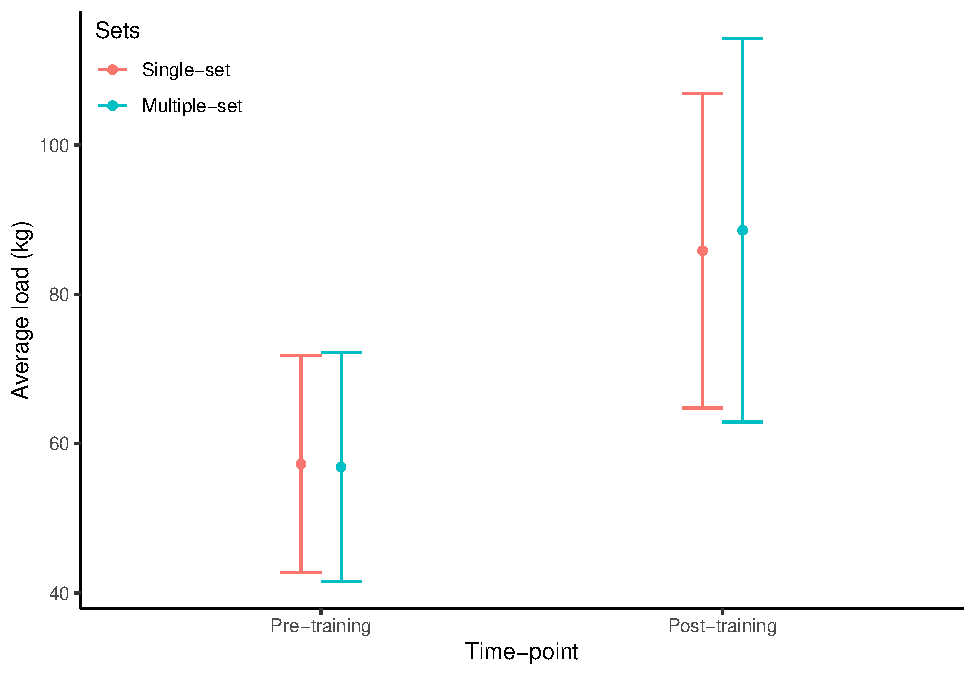
\includegraphics{_main_files/figure-latex/unnamed-chunk-6-1.pdf}
\caption{\label{fig:unnamed-chunk-6}Figuren viser økning i muskelstyrke mellom multiple- sett og singe- sett ved pretest og posttest etter 12 uker med styrketrening (P= 0.029, diff= -0.029)}
\end{figure}

\begin{figure}
\centering
\includegraphics{_main_files/figure-latex/Prosentvis økning figur styrke-1.pdf}
\caption{(\#fig:Prosentvis økning figur styrke)Figuren viser prosentvis økning i muskelstyrke mellom multiple- sett og singe- sett ved posttest etter 12 uker med styrketrening (P- 0.029)}
\end{figure}

\hypertarget{diskusjon}{%
\section{Diskusjon}\label{diskusjon}}

I denne studien viste det at multiple- sett styrketrening førte til bedre økning i muskelstyrke enn single- sett trening. Dette resultatet stemmer overns med andre studier som har funnet at flere sett er bedre enn en \citep{galvão2005e, humburg2007c}.

Likevel samsvarer ikke resultatet i denne studien med \citep{carpinelli1998d}. Der kom de frem til at det ikke var noen signifikant forskjell i størrelsen på styrke økningen mellom 1- sett og multiple sett. I studien til \citep{carpinelli1998b} så de på studien til \citep{reid1987a} som fant ut at den gjennomsnittlige økningen i styrke var på 17,7\% for single- sett gruppen og på 17,9\% multiple- sett. Sammenlignet med vårt resultat som var på henholdsvis 25\% og 31\% på single- sett og multiple- sett. Disse forskjellene i konklusjon kan muligens bli forklart av \citep{galvão2005d} konkluderer med at styrketrening med single- sett øvelser er nok til å signifikant øke muskel funksjon, selv om muskelstyrke vil bli bedre ved et høyere treningsvolum som multiple- sett gir.

\hypertarget{konklusjon}{%
\subsection{Konklusjon}\label{konklusjon}}

Totalt sett viste denne studien at multiple- sett ga en bedre økning i muskelstyrke sammenlignet med single- sett. Selv om begge gruppene hadde økning vil det kunne være mer hensiktsmessig å trene styrketrening med multiple- sett.

  \bibliography{book.bib}

\end{document}
